\documentclass[aspectratio=169,11pt]{beamer}
% =====================================================================
%  pds-beamer.tex — Estilo común de las transparencias.
%
%  Uso (desde teoría/Tx/transparencias/):
%     \documentclass[aspectratio=169,11pt]{beamer}
%     % =====================================================================
%  pds-beamer.tex — Estilo común de las transparencias.
%
%  Uso (desde teoría/Tx/transparencias/):
%     \documentclass[aspectratio=169,11pt]{beamer}
%     % =====================================================================
%  pds-beamer.tex — Estilo común de las transparencias.
%
%  Uso (desde teoría/Tx/transparencias/):
%     \documentclass[aspectratio=169,11pt]{beamer}
%     \input{../../comun/pds-beamer}
%     \title{...}  \subtitle{Tema x · ...}
%     \begin{document}
%       \portada
%       ...
%     \end{document}
%  Compilar con:  latexmk -xelatex  (o «make» desde teoría/)
% =====================================================================

\usetheme{Boadilla}
\usecolortheme{orchid}
\usefonttheme{professionalfonts}
\setbeamercovered{transparent}
\setbeamersize{text margin left=0.8cm, text margin right=0.8cm}
\setbeamertemplate{navigation symbols}{}
\setbeamertemplate{itemize item}[square]
\setbeamertemplate{itemize subitem}[circle]
\setbeamertemplate{itemize subsubitem}[triangle]
\setbeamertemplate{enumerate item}[square]
\setbeamertemplate{enumerate subitem}[circle]
\setbeamertemplate{caption}{\raggedright\insertcaption\par}

\input{../../comun/pds-comun.tex}

% Tipografía: Fira Sans + Fira Math (legibles en proyector)
\usepackage{fontspec}
\usepackage{unicode-math}
% Se cargan por nombre de fichero para que funcionen con cualquier
% instalación de TeX Live (o MiKTeX) sin instalar fuentes en el sistema.
\setmainfont{FiraSans}[Extension=.otf, UprightFont=*-Regular, BoldFont=*-SemiBold,
  ItalicFont=*-Italic, BoldItalicFont=*-SemiBoldItalic]
\setsansfont{FiraSans}[Extension=.otf, UprightFont=*-Regular, BoldFont=*-SemiBold,
  ItalicFont=*-Italic, BoldItalicFont=*-SemiBoldItalic]
\setmonofont{FiraMono}[Extension=.otf, UprightFont=*-Regular, BoldFont=*-Medium, AutoFakeSlant=0.15, Scale=0.92]
\setmathfont{FiraMath-Regular.otf}
\setmathfont{latinmodern-math.otf}[range={"229B,"22EE,"22F1}]

% Colores del tema ajustados a la paleta común (más contraste)
\setbeamercolor{structure}{fg=pdsazul}
\setbeamercolor{alerted text}{fg=pdsrojo}
\setbeamercolor{example text}{fg=pdsverde}
\setbeamercolor{block title}{bg=pdsazul, fg=white}
\setbeamercolor{block body}{bg=pdsfondo}
\setbeamercolor{block title alerted}{bg=pdsrojo, fg=white}
\setbeamercolor{block body alerted}{bg=pdsrojo!6}
\setbeamercolor{block title example}{bg=pdsverde, fg=white}
\setbeamercolor{block body example}{bg=pdsverde!6}
\setbeamercolor{frametitle}{fg=pdsazul, bg=white}
\setbeamerfont{frametitle}{size=\large, series=\bfseries}
\setbeamerfont{block title}{size=\normalsize, series=\bfseries}
\setbeamertemplate{blocks}[rounded][shadow=false]

% Logo en la esquina superior derecha de cada transparencia
\pgfdeclareimage[height=0.8cm]{logo}{../../comun/ucm.png}
\addtobeamertemplate{frametitle}{}{%
  \begin{tikzpicture}[remember picture, overlay]
    \node[anchor=north east, inner sep=0pt] at ([xshift=-0.25cm, yshift=-0.2cm]current page.north east) {\pgfuseimage{logo}};
  \end{tikzpicture}}

% Datos de portada
\author[\autorescorto]{\autores}
\institute[UCM]{\footnotesize\departamento\\\universidad}
\date[\curso]{\footnotesize\grado\\\curso}

\newcommand{\portada}{%
  \begin{frame}[plain]
    \begin{center}
      
\includegraphics[height=1.9cm]{../../comun/ucm.png}
    \end{center}
    \vspace{-0.4cm}
    \titlepage
  \end{frame}}

% Índice al empezar cada sección
\AtBeginSection[]{%
  \begin{frame}{Contenido}
    \tableofcontents[currentsection, hideothersubsections]
  \end{frame}}

\renewcommand{\pdscodesize}{\scriptsize}

% Utilidades
% \herramienta{T1-convolucion-continua}: enlace a la página publicada de
% herramientas/html (se abre en el navegador, sin instalar nada).
% \herramientaservidor{server/....py}: app que necesita Python (bokeh serve).
\newcommand{\urlherramientas}{https://ucm-237.github.io/PdS/}
\newcommand{\herramienta}[1]{%
  \par\vfill\hfill{\scriptsize\color{pdsgris}\faIcon\ \href{\urlherramientas#1.html}{Herramienta interactiva: \texttt{#1}}}}
\newcommand{\herramientaservidor}[1]{%
  \par\vfill\hfill{\scriptsize\color{pdsgris}\faIcon\ Herramienta interactiva (con Python): \texttt{herramientas/#1}}}
\newcommand{\faIcon}{\textbf{▶}}
\newcommand{\gris}[1]{{\color{pdsgris}#1}}
\newcommand{\nota}[1]{\par\vspace{2pt}{\footnotesize\color{pdsgris}\textit{#1}}\par}
% Nota sobre una errata de versiones anteriores (solo con \ERRATAS)
\newcommand{\errata}[1]{\iferratas\nota{Errata de versiones anteriores: #1}\fi}
\newcommand{\apuntes}[1]{\nota{Más detalle en los apuntes, #1.}}

% Bloques con nombre en castellano
\newenvironment{definicion}[1][Definición]{\begin{block}{#1}}{\end{block}}
\newenvironment{importante}[1][Importante]{\begin{alertblock}{#1}}{\end{alertblock}}
\newenvironment{ejemplo}[1][Ejemplo]{\begin{exampleblock}{#1}}{\end{exampleblock}}

%     \title{...}  \subtitle{Tema x · ...}
%     \begin{document}
%       \portada
%       ...
%     \end{document}
%  Compilar con:  latexmk -xelatex  (o «make» desde teoría/)
% =====================================================================

\usetheme{Boadilla}
\usecolortheme{orchid}
\usefonttheme{professionalfonts}
\setbeamercovered{transparent}
\setbeamersize{text margin left=0.8cm, text margin right=0.8cm}
\setbeamertemplate{navigation symbols}{}
\setbeamertemplate{itemize item}[square]
\setbeamertemplate{itemize subitem}[circle]
\setbeamertemplate{itemize subsubitem}[triangle]
\setbeamertemplate{enumerate item}[square]
\setbeamertemplate{enumerate subitem}[circle]
\setbeamertemplate{caption}{\raggedright\insertcaption\par}

% =====================================================================
%  pds-comun.tex — Paquetes, colores y estilos de código comunes a
%  transparencias, apuntes y hojas de ejercicios. Compilar con XeLaTeX.
%  No cargar directamente: lo cargan pds-beamer.tex y pds-apuntes.tex.
% =====================================================================

\usepackage{polyglossia}
\setmainlanguage{spanish}
\usepackage{mathtools}
\usepackage{graphicx}
\usepackage{booktabs}
\usepackage{multirow}
\usepackage{array}
\usepackage{xcolor}
\usepackage{tikz}
\usetikzlibrary{positioning,arrows.meta,calc,shapes.geometric,decorations.pathreplacing}
\usepackage{listings}
\usepackage{siunitx}
\sisetup{output-decimal-marker={,}, group-separator={\,}, per-mode=symbol}

% Notas de erratas de versiones anteriores: no se imprimen salvo que se
% defina \ERRATAS antes de cargar el estilo (make ERRATAS=1)
\newif\iferratas
\ifdefined\ERRATAS \erratastrue \fi

% Ruta común (logo y figuras compartidas)
\providecommand{\rutacomun}{../../comun/}
\input{\rutacomun datos.tex}

% ---------------------------------------------------------------------
%  Paleta (la misma que usan las figuras generadas con Python,
%  ver comun/pds_estilo.py)
% ---------------------------------------------------------------------
\definecolor{pdsazul}{HTML}{2B3A8C}
\definecolor{pdsrojo}{HTML}{C0392B}
\definecolor{pdsverde}{HTML}{1E7B4F}
\definecolor{pdsnaranja}{HTML}{D9822B}
\definecolor{pdsgris}{HTML}{5A5A66}
\definecolor{pdsfondo}{HTML}{F3F4FA}
\definecolor{pdscodigo}{HTML}{F7F7F2}

% ---------------------------------------------------------------------
%  Diagramas de bloques (TikZ)
% ---------------------------------------------------------------------
\tikzset{
  bloque/.style={rectangle, rounded corners=2pt, draw=pdsazul!80, fill=pdsfondo,
                 very thick, minimum height=8mm, minimum width=14mm, align=center},
  sumador/.style={circle, draw=pdsazul!80, fill=pdsfondo, thick, inner sep=1.5pt},
  flecha/.style={-{Stealth[length=2.2mm]}, thick, pdsgris},
}

% ---------------------------------------------------------------------
%  Código: Python y Matlab en paralelo
% ---------------------------------------------------------------------
\newcommand{\pdscodesize}{\footnotesize}
\lstdefinestyle{pds}{
  basicstyle=\ttfamily\pdscodesize,
  keywordstyle=\color{pdsazul}\bfseries,
  commentstyle=\color{pdsverde}\itshape,
  stringstyle=\color{pdsrojo},
  numbers=none,
  backgroundcolor=\color{pdscodigo},
  frame=single, rulecolor=\color{pdsgris!40}, framerule=0.4pt,
  xleftmargin=2pt, xrightmargin=2pt, aboveskip=2pt, belowskip=2pt,
  columns=fullflexible, keepspaces=true,
  showstringspaces=false, breaklines=true, tabsize=4,
  upquote=true,
  % Con XeLaTeX, listings desordena los caracteres no ASCII junto a
  % dígitos («2π» sale «π2»): se sustituyen por su versión matemática.
  literate={π}{{$\pi$}}1 {δ}{{$\delta$}}1 {ω}{{$\omega$}}1 {Ω}{{$\Omega$}}1
           {≈}{{$\approx$}}1 {µ}{{$\mu$}}1 {·}{{$\cdot$}}1 {α}{{$\alpha$}}1
           {á}{{á}}1 {é}{{é}}1 {í}{{í}}1 {ó}{{ó}}1 {ú}{{ú}}1 {ñ}{{ñ}}1 {¿}{{¿}}1,
}
\lstdefinestyle{python}{style=pds, language=Python,
  morekeywords={as,True,False,None}}
\lstdefinestyle{matlab}{style=pds, language=Matlab,
  morekeywords={function,end,true,false}}

% \codigo{<ruta sin extensión>} muestra el mismo ejemplo en Python
% y en Matlab, uno al lado del otro. Los ficheros viven en
% ../codigo/python/<nombre>.py y ../codigo/matlab/<nombre>.m y se
% ejecutan en las pruebas (make prueba-codigo).
\newcommand{\rutacodigo}{../codigo/}
\newcommand{\codigoetiqueta}[1]{{\sffamily\scriptsize\bfseries\color{pdsgris}#1}}
\newcommand{\codigo}[2][]{%
  \par\noindent
  \begin{minipage}[t]{0.495\linewidth}
    \codigoetiqueta{Python}\par\vspace{1pt}
    \lstinputlisting[style=python,#1]{\rutacodigo python/#2.py}
  \end{minipage}\hfill
  \begin{minipage}[t]{0.495\linewidth}
    \codigoetiqueta{Matlab}\par\vspace{1pt}
    \lstinputlisting[style=matlab,#1]{\rutacodigo matlab/#2.m}
  \end{minipage}\par}

\input{\rutacomun notacion.tex}


% Tipografía: Fira Sans + Fira Math (legibles en proyector)
\usepackage{fontspec}
\usepackage{unicode-math}
% Se cargan por nombre de fichero para que funcionen con cualquier
% instalación de TeX Live (o MiKTeX) sin instalar fuentes en el sistema.
\setmainfont{FiraSans}[Extension=.otf, UprightFont=*-Regular, BoldFont=*-SemiBold,
  ItalicFont=*-Italic, BoldItalicFont=*-SemiBoldItalic]
\setsansfont{FiraSans}[Extension=.otf, UprightFont=*-Regular, BoldFont=*-SemiBold,
  ItalicFont=*-Italic, BoldItalicFont=*-SemiBoldItalic]
\setmonofont{FiraMono}[Extension=.otf, UprightFont=*-Regular, BoldFont=*-Medium, AutoFakeSlant=0.15, Scale=0.92]
\setmathfont{FiraMath-Regular.otf}
\setmathfont{latinmodern-math.otf}[range={"229B,"22EE,"22F1}]

% Colores del tema ajustados a la paleta común (más contraste)
\setbeamercolor{structure}{fg=pdsazul}
\setbeamercolor{alerted text}{fg=pdsrojo}
\setbeamercolor{example text}{fg=pdsverde}
\setbeamercolor{block title}{bg=pdsazul, fg=white}
\setbeamercolor{block body}{bg=pdsfondo}
\setbeamercolor{block title alerted}{bg=pdsrojo, fg=white}
\setbeamercolor{block body alerted}{bg=pdsrojo!6}
\setbeamercolor{block title example}{bg=pdsverde, fg=white}
\setbeamercolor{block body example}{bg=pdsverde!6}
\setbeamercolor{frametitle}{fg=pdsazul, bg=white}
\setbeamerfont{frametitle}{size=\large, series=\bfseries}
\setbeamerfont{block title}{size=\normalsize, series=\bfseries}
\setbeamertemplate{blocks}[rounded][shadow=false]

% Logo en la esquina superior derecha de cada transparencia
\pgfdeclareimage[height=0.8cm]{logo}{../../comun/ucm.png}
\addtobeamertemplate{frametitle}{}{%
  \begin{tikzpicture}[remember picture, overlay]
    \node[anchor=north east, inner sep=0pt] at ([xshift=-0.25cm, yshift=-0.2cm]current page.north east) {\pgfuseimage{logo}};
  \end{tikzpicture}}

% Datos de portada
\author[\autorescorto]{\autores}
\institute[UCM]{\footnotesize\departamento\\\universidad}
\date[\curso]{\footnotesize\grado\\\curso}

\newcommand{\portada}{%
  \begin{frame}[plain]
    \begin{center}
      
\includegraphics[height=1.9cm]{../../comun/ucm.png}
    \end{center}
    \vspace{-0.4cm}
    \titlepage
  \end{frame}}

% Índice al empezar cada sección
\AtBeginSection[]{%
  \begin{frame}{Contenido}
    \tableofcontents[currentsection, hideothersubsections]
  \end{frame}}

\renewcommand{\pdscodesize}{\scriptsize}

% Utilidades
% \herramienta{T1-convolucion-continua}: enlace a la página publicada de
% herramientas/html (se abre en el navegador, sin instalar nada).
% \herramientaservidor{server/....py}: app que necesita Python (bokeh serve).
\newcommand{\urlherramientas}{https://ucm-237.github.io/PdS/}
\newcommand{\herramienta}[1]{%
  \par\vfill\hfill{\scriptsize\color{pdsgris}\faIcon\ \href{\urlherramientas#1.html}{Herramienta interactiva: \texttt{#1}}}}
\newcommand{\herramientaservidor}[1]{%
  \par\vfill\hfill{\scriptsize\color{pdsgris}\faIcon\ Herramienta interactiva (con Python): \texttt{herramientas/#1}}}
\newcommand{\faIcon}{\textbf{▶}}
\newcommand{\gris}[1]{{\color{pdsgris}#1}}
\newcommand{\nota}[1]{\par\vspace{2pt}{\footnotesize\color{pdsgris}\textit{#1}}\par}
% Nota sobre una errata de versiones anteriores (solo con \ERRATAS)
\newcommand{\errata}[1]{\iferratas\nota{Errata de versiones anteriores: #1}\fi}
\newcommand{\apuntes}[1]{\nota{Más detalle en los apuntes, #1.}}

% Bloques con nombre en castellano
\newenvironment{definicion}[1][Definición]{\begin{block}{#1}}{\end{block}}
\newenvironment{importante}[1][Importante]{\begin{alertblock}{#1}}{\end{alertblock}}
\newenvironment{ejemplo}[1][Ejemplo]{\begin{exampleblock}{#1}}{\end{exampleblock}}

%     \title{...}  \subtitle{Tema x · ...}
%     \begin{document}
%       \portada
%       ...
%     \end{document}
%  Compilar con:  latexmk -xelatex  (o «make» desde teoría/)
% =====================================================================

\usetheme{Boadilla}
\usecolortheme{orchid}
\usefonttheme{professionalfonts}
\setbeamercovered{transparent}
\setbeamersize{text margin left=0.8cm, text margin right=0.8cm}
\setbeamertemplate{navigation symbols}{}
\setbeamertemplate{itemize item}[square]
\setbeamertemplate{itemize subitem}[circle]
\setbeamertemplate{itemize subsubitem}[triangle]
\setbeamertemplate{enumerate item}[square]
\setbeamertemplate{enumerate subitem}[circle]
\setbeamertemplate{caption}{\raggedright\insertcaption\par}

% =====================================================================
%  pds-comun.tex — Paquetes, colores y estilos de código comunes a
%  transparencias, apuntes y hojas de ejercicios. Compilar con XeLaTeX.
%  No cargar directamente: lo cargan pds-beamer.tex y pds-apuntes.tex.
% =====================================================================

\usepackage{polyglossia}
\setmainlanguage{spanish}
\usepackage{mathtools}
\usepackage{graphicx}
\usepackage{booktabs}
\usepackage{multirow}
\usepackage{array}
\usepackage{xcolor}
\usepackage{tikz}
\usetikzlibrary{positioning,arrows.meta,calc,shapes.geometric,decorations.pathreplacing}
\usepackage{listings}
\usepackage{siunitx}
\sisetup{output-decimal-marker={,}, group-separator={\,}, per-mode=symbol}

% Notas de erratas de versiones anteriores: no se imprimen salvo que se
% defina \ERRATAS antes de cargar el estilo (make ERRATAS=1)
\newif\iferratas
\ifdefined\ERRATAS \erratastrue \fi

% Ruta común (logo y figuras compartidas)
\providecommand{\rutacomun}{../../comun/}
\input{\rutacomun datos.tex}

% ---------------------------------------------------------------------
%  Paleta (la misma que usan las figuras generadas con Python,
%  ver comun/pds_estilo.py)
% ---------------------------------------------------------------------
\definecolor{pdsazul}{HTML}{2B3A8C}
\definecolor{pdsrojo}{HTML}{C0392B}
\definecolor{pdsverde}{HTML}{1E7B4F}
\definecolor{pdsnaranja}{HTML}{D9822B}
\definecolor{pdsgris}{HTML}{5A5A66}
\definecolor{pdsfondo}{HTML}{F3F4FA}
\definecolor{pdscodigo}{HTML}{F7F7F2}

% ---------------------------------------------------------------------
%  Diagramas de bloques (TikZ)
% ---------------------------------------------------------------------
\tikzset{
  bloque/.style={rectangle, rounded corners=2pt, draw=pdsazul!80, fill=pdsfondo,
                 very thick, minimum height=8mm, minimum width=14mm, align=center},
  sumador/.style={circle, draw=pdsazul!80, fill=pdsfondo, thick, inner sep=1.5pt},
  flecha/.style={-{Stealth[length=2.2mm]}, thick, pdsgris},
}

% ---------------------------------------------------------------------
%  Código: Python y Matlab en paralelo
% ---------------------------------------------------------------------
\newcommand{\pdscodesize}{\footnotesize}
\lstdefinestyle{pds}{
  basicstyle=\ttfamily\pdscodesize,
  keywordstyle=\color{pdsazul}\bfseries,
  commentstyle=\color{pdsverde}\itshape,
  stringstyle=\color{pdsrojo},
  numbers=none,
  backgroundcolor=\color{pdscodigo},
  frame=single, rulecolor=\color{pdsgris!40}, framerule=0.4pt,
  xleftmargin=2pt, xrightmargin=2pt, aboveskip=2pt, belowskip=2pt,
  columns=fullflexible, keepspaces=true,
  showstringspaces=false, breaklines=true, tabsize=4,
  upquote=true,
  % Con XeLaTeX, listings desordena los caracteres no ASCII junto a
  % dígitos («2π» sale «π2»): se sustituyen por su versión matemática.
  literate={π}{{$\pi$}}1 {δ}{{$\delta$}}1 {ω}{{$\omega$}}1 {Ω}{{$\Omega$}}1
           {≈}{{$\approx$}}1 {µ}{{$\mu$}}1 {·}{{$\cdot$}}1 {α}{{$\alpha$}}1
           {á}{{á}}1 {é}{{é}}1 {í}{{í}}1 {ó}{{ó}}1 {ú}{{ú}}1 {ñ}{{ñ}}1 {¿}{{¿}}1,
}
\lstdefinestyle{python}{style=pds, language=Python,
  morekeywords={as,True,False,None}}
\lstdefinestyle{matlab}{style=pds, language=Matlab,
  morekeywords={function,end,true,false}}

% \codigo{<ruta sin extensión>} muestra el mismo ejemplo en Python
% y en Matlab, uno al lado del otro. Los ficheros viven en
% ../codigo/python/<nombre>.py y ../codigo/matlab/<nombre>.m y se
% ejecutan en las pruebas (make prueba-codigo).
\newcommand{\rutacodigo}{../codigo/}
\newcommand{\codigoetiqueta}[1]{{\sffamily\scriptsize\bfseries\color{pdsgris}#1}}
\newcommand{\codigo}[2][]{%
  \par\noindent
  \begin{minipage}[t]{0.495\linewidth}
    \codigoetiqueta{Python}\par\vspace{1pt}
    \lstinputlisting[style=python,#1]{\rutacodigo python/#2.py}
  \end{minipage}\hfill
  \begin{minipage}[t]{0.495\linewidth}
    \codigoetiqueta{Matlab}\par\vspace{1pt}
    \lstinputlisting[style=matlab,#1]{\rutacodigo matlab/#2.m}
  \end{minipage}\par}

\input{\rutacomun notacion.tex}


% Tipografía: Fira Sans + Fira Math (legibles en proyector)
\usepackage{fontspec}
\usepackage{unicode-math}
% Se cargan por nombre de fichero para que funcionen con cualquier
% instalación de TeX Live (o MiKTeX) sin instalar fuentes en el sistema.
\setmainfont{FiraSans}[Extension=.otf, UprightFont=*-Regular, BoldFont=*-SemiBold,
  ItalicFont=*-Italic, BoldItalicFont=*-SemiBoldItalic]
\setsansfont{FiraSans}[Extension=.otf, UprightFont=*-Regular, BoldFont=*-SemiBold,
  ItalicFont=*-Italic, BoldItalicFont=*-SemiBoldItalic]
\setmonofont{FiraMono}[Extension=.otf, UprightFont=*-Regular, BoldFont=*-Medium, AutoFakeSlant=0.15, Scale=0.92]
\setmathfont{FiraMath-Regular.otf}
\setmathfont{latinmodern-math.otf}[range={"229B,"22EE,"22F1}]

% Colores del tema ajustados a la paleta común (más contraste)
\setbeamercolor{structure}{fg=pdsazul}
\setbeamercolor{alerted text}{fg=pdsrojo}
\setbeamercolor{example text}{fg=pdsverde}
\setbeamercolor{block title}{bg=pdsazul, fg=white}
\setbeamercolor{block body}{bg=pdsfondo}
\setbeamercolor{block title alerted}{bg=pdsrojo, fg=white}
\setbeamercolor{block body alerted}{bg=pdsrojo!6}
\setbeamercolor{block title example}{bg=pdsverde, fg=white}
\setbeamercolor{block body example}{bg=pdsverde!6}
\setbeamercolor{frametitle}{fg=pdsazul, bg=white}
\setbeamerfont{frametitle}{size=\large, series=\bfseries}
\setbeamerfont{block title}{size=\normalsize, series=\bfseries}
\setbeamertemplate{blocks}[rounded][shadow=false]

% Logo en la esquina superior derecha de cada transparencia
\pgfdeclareimage[height=0.8cm]{logo}{../../comun/ucm.png}
\addtobeamertemplate{frametitle}{}{%
  \begin{tikzpicture}[remember picture, overlay]
    \node[anchor=north east, inner sep=0pt] at ([xshift=-0.25cm, yshift=-0.2cm]current page.north east) {\pgfuseimage{logo}};
  \end{tikzpicture}}

% Datos de portada
\author[\autorescorto]{\autores}
\institute[UCM]{\footnotesize\departamento\\\universidad}
\date[\curso]{\footnotesize\grado\\\curso}

\newcommand{\portada}{%
  \begin{frame}[plain]
    \begin{center}
      
\includegraphics[height=1.9cm]{../../comun/ucm.png}
    \end{center}
    \vspace{-0.4cm}
    \titlepage
  \end{frame}}

% Índice al empezar cada sección
\AtBeginSection[]{%
  \begin{frame}{Contenido}
    \tableofcontents[currentsection, hideothersubsections]
  \end{frame}}

\renewcommand{\pdscodesize}{\scriptsize}

% Utilidades
% \herramienta{T1-convolucion-continua}: enlace a la página publicada de
% herramientas/html (se abre en el navegador, sin instalar nada).
% \herramientaservidor{server/....py}: app que necesita Python (bokeh serve).
\newcommand{\urlherramientas}{https://ucm-237.github.io/PdS/}
\newcommand{\herramienta}[1]{%
  \par\vfill\hfill{\scriptsize\color{pdsgris}\faIcon\ \href{\urlherramientas#1.html}{Herramienta interactiva: \texttt{#1}}}}
\newcommand{\herramientaservidor}[1]{%
  \par\vfill\hfill{\scriptsize\color{pdsgris}\faIcon\ Herramienta interactiva (con Python): \texttt{herramientas/#1}}}
\newcommand{\faIcon}{\textbf{▶}}
\newcommand{\gris}[1]{{\color{pdsgris}#1}}
\newcommand{\nota}[1]{\par\vspace{2pt}{\footnotesize\color{pdsgris}\textit{#1}}\par}
% Nota sobre una errata de versiones anteriores (solo con \ERRATAS)
\newcommand{\errata}[1]{\iferratas\nota{Errata de versiones anteriores: #1}\fi}
\newcommand{\apuntes}[1]{\nota{Más detalle en los apuntes, #1.}}

% Bloques con nombre en castellano
\newenvironment{definicion}[1][Definición]{\begin{block}{#1}}{\end{block}}
\newenvironment{importante}[1][Importante]{\begin{alertblock}{#1}}{\end{alertblock}}
\newenvironment{ejemplo}[1][Ejemplo]{\begin{exampleblock}{#1}}{\end{exampleblock}}

\graphicspath{{../figuras/}}

\title[T5 · STFT]{Aplicaciones}
\subtitle{Tema 5 · Parte 1: transformada de Fourier de tiempo corto y espectrograma}

\begin{document}
\portada

\begin{frame}{Objetivos del tema}
  \begin{itemize}
    \item Aplicar lo visto en los temas anteriores (DFT, ventanas, filtros) a señales reales.
    \item \alert{Señales no estacionarias}: ver cómo cambia el espectro con el tiempo mediante la transformada de Fourier de tiempo corto (STFT) y el espectrograma.
    \item \alert{Wavelets}: análisis a varias escalas, transformada continua y discreta, bancos de filtros; eliminación de ruido y compresión.
    \item \alert{Imágenes}: señales bidimensionales, histograma, convolución 2D, DFT 2D y filtrado en frecuencia.
  \end{itemize}
  \bigskip
  \gris{Partes: 1 STFT y espectrograma · 2 Wavelets · 3 Procesamiento de imágenes.}
\end{frame}

% =====================================================================
\section{Señales no estacionarias}

\begin{frame}{¿Qué le falta a la DFT?}
  \begin{columns}[c]
    \begin{column}{0.4\textwidth}
      \small
      \begin{itemize}
        \item La DFT de una señal entera dice \alert{qué} frecuencias hay, pero no \alert{cuándo} aparecen.
        \item Las señales reales cambian: voz, música, vibraciones de una máquina que arranca, radar, sismos.
        \item $x_1$ y $x_2$ tienen los mismos tonos en orden inverso: sus módulos de la DFT coinciden. La diferencia está en la fase, que es imposible de leer a simple vista.
      \end{itemize}
    \end{column}
    \begin{column}{0.58\textwidth}
      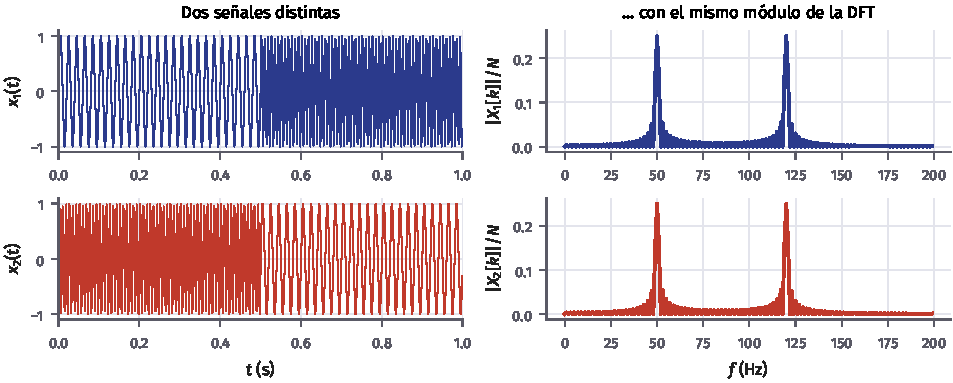
\includegraphics[width=\linewidth]{no_estacionaria}
    \end{column}
  \end{columns}
\end{frame}

\begin{frame}{Idea: analizar la señal por tramos}
  \begin{center}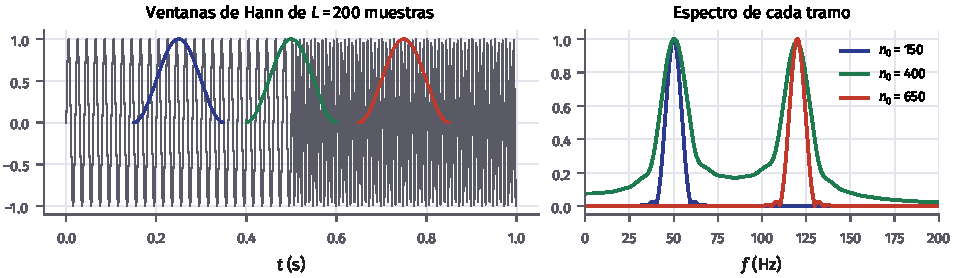
\includegraphics[width=0.85\linewidth]{stft_tramos}\end{center}
  \small
  \begin{itemize}
    \item Se multiplica la señal por una \alert{ventana} $w[n]$ de $L$ muestras centrada en cada instante y se calcula la DFT del tramo.
    \item Truncar es multiplicar por una ventana: el espectro del tramo es la convolución del espectro de la señal con el de la ventana (tema~3). Por eso se usan ventanas suaves (Hann, Hamming) y no la rectangular.
    \item El tramo verde contiene el cambio de 50 a 120\,Hz y muestra los dos tonos.
  \end{itemize}
\end{frame}

% =====================================================================
\section{Transformada de Fourier de tiempo corto}

\begin{frame}{Definición}
  \small
  \begin{definicion}[STFT]
    Continua, con ventana $w(t)$ desplazada a $\tau$:
    \[
      X(\tau,\omega)=\int_{-\infty}^{\infty}x(t)\,w(t-\tau)\,\e^{-j\omega t}\dd t .
    \]
    Discreta, con salto $R$ entre tramos y $N\ge L$ puntos de DFT:
    \[
      X[m,k]=\sum_{n=-\infty}^{\infty}x[n]\,w[n-mR]\,\e^{-j2\pi kn/N},\qquad k=0,\dots,N-1 .
    \]
  \end{definicion}
  \small
  \begin{itemize}
    \item Para cada $m$ (tramo) hay un espectro; para cada $k$ (frecuencia), una señal en el tiempo.
    \item Es una función de \alert{dos variables}: tiempo y frecuencia. El tramo $m$ está centrado en $t_m=(mR+L/2)/f_s$ y el índice $k$ corresponde a $f_k=kf_s/N$. Si se escribe $\e^{-j2\pi k(n-mR)/N}$ cambia la fase, no el módulo.
  \end{itemize}
\end{frame}

\begin{frame}{Parámetros}
  \begin{columns}[T]
    \begin{column}{0.55\textwidth}
      \small
      \begin{itemize}
        \item \alert{Longitud de ventana $L$}: fija la resolución. Duración $\Delta t=L/f_s$.
        \item \alert{Tipo de ventana}: el lóbulo principal de Hann mide $4f_s/L$ entre ceros; dos tonos se separan si distan más de $\approx2f_s/L$.
        \item \alert{Salto $R$} (o solapamiento $L-R$): cada cuántas muestras se calcula un espectro. Con $R<L$ los tramos se solapan; típicamente 50–75\,\%.
        \item \alert{Puntos de la DFT $N\ge L$}: rellenar con ceros interpola el espectro, pero no mejora la resolución.
      \end{itemize}
    \end{column}
    \begin{column}{0.42\textwidth}
      \begin{importante}[Número de tramos]
        Para una señal de $N_x$ muestras:
        \[
          M=\left\lfloor\frac{N_x-L}{R}\right\rfloor+1 .
        \]
      \end{importante}
      \footnotesize
      $f_s=1$\,kHz, 2\,s, $L=128$, $R=32$: $M=59$ tramos de $N/2+1=129$ frecuencias con $N=256$.
    \end{column}
  \end{columns}
\end{frame}

\begin{frame}{Espectrograma}
  \begin{center}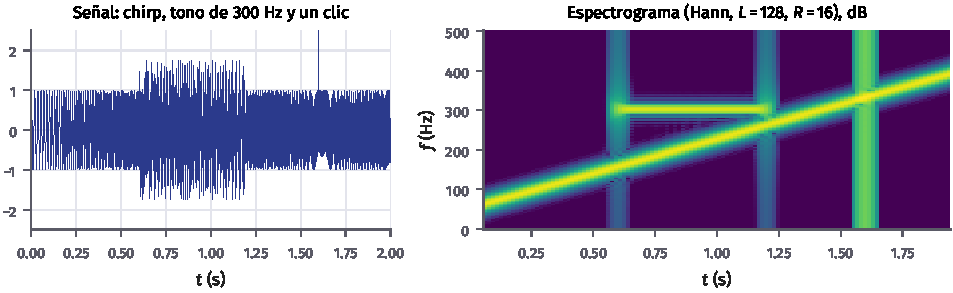
\includegraphics[width=0.95\linewidth]{espectrograma_ejemplo}\end{center}
  \small
  \begin{itemize}
    \item El \alert{espectrograma} es $\abs{X[m,k]}^2$ representado en el plano tiempo-frecuencia con un mapa de colores, normalmente en dB.
    \item Se ven el chirp (recta), el tono de 300\,Hz entre 0,6 y 1,2\,s y el clic (línea vertical: un impulso contiene todas las frecuencias).
  \end{itemize}
  \herramienta{T5-stft}
\end{frame}

\begin{frame}{En código: STFT paso a paso}
  \codigo[basicstyle=\ttfamily\fontsize{6.8}{7.8}\selectfont]{stft_manual}
  \nota{Matlab: \texttt{spectrogram(x, w, L-R, N, fs)}; Python: \texttt{scipy.signal.spectrogram} o \texttt{ShortTimeFFT}. Octave no tiene \texttt{spectrogram}, pero sí \texttt{specgram}.}
\end{frame}

% =====================================================================
\section{Resolución en tiempo y en frecuencia}

\begin{frame}{El compromiso tiempo-frecuencia}
  \begin{center}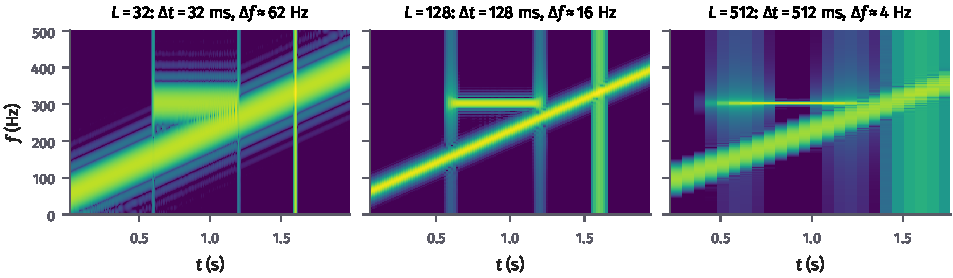
\includegraphics[width=\linewidth]{resolucion_tf}\end{center}
  \small
  \begin{itemize}
    \item Ventana corta: el clic y los bordes del tono se localizan bien, pero las frecuencias se emborronan.
    \item Ventana larga: el tono de 300\,Hz es una raya fina, pero el chirp se ensancha y el clic se extiende medio segundo.
  \end{itemize}
\end{frame}

\begin{frame}{Principio de incertidumbre}
  \begin{columns}[c]
    \begin{column}{0.56\textwidth}
      \small
      \begin{itemize}
        \item Una ventana de duración $\Delta t$ tiene un espectro de anchura $\Delta f\sim1/\Delta t$:
        \[
          \Delta t\cdot\Delta f\ge\text{constante}.
        \]
        \item Con desviaciones típicas de $\abs{w(t)}^2$ y $\abs{W(j\omega)}^2$, $\sigma_t\sigma_\omega\ge\frac12$, con igualdad para la ventana gaussiana.
        \item No se puede tener a la vez resolución fina en tiempo y en frecuencia. La STFT usa la \alert{misma} resolución en todo el plano.
        \item Elegir $L$ depende de la señal: para voz, 20–30\,ms (el tracto vocal cambia más despacio); para música, más larga.
      \end{itemize}
    \end{column}
    \begin{column}{0.4\textwidth}
      \begin{ejemplo}[Dos tonos y dos clics]
        \footnotesize
        $f_s=1$\,kHz. Separar dos tonos a 20\,Hz con Hann pide $L\ge2f_s/20=100$ muestras (100\,ms). Separar dos clics a 10\,ms pide $L\lesssim10$. No hay $L$ que cumpla ambas cosas: hacen falta dos espectrogramas o una wavelet (parte~2).
      \end{ejemplo}
    \end{column}
  \end{columns}
  \herramienta{T5-resolucion-tiempo-frecuencia}
\end{frame}

% =====================================================================
\section{Síntesis: volver al tiempo}

\begin{frame}{Solapamiento y suma}
  \begin{columns}[c]
    \begin{column}{0.56\textwidth}
      \small
      \begin{itemize}
        \item La IDFT de cada tramo da $x[n]w[n-mR]$. Si las ventanas desplazadas suman una constante,
        \[
          \sum_m w[n-mR]=C\quad\forall n ,
        \]
        (condición \alert{COLA}), sumar los tramos devuelve $Cx[n]$: \alert{solapamiento y suma} (\emph{overlap-add}).
        \item Hann periódica con $R=L/2$ o $L/4$, Hamming con $R=L/2$ y rectangular con $R=L$ cumplen COLA.
        \item Así se modifica la señal en el plano tiempo-frecuencia y se vuelve al tiempo.
      \end{itemize}
    \end{column}
    \begin{column}{0.42\textwidth}
      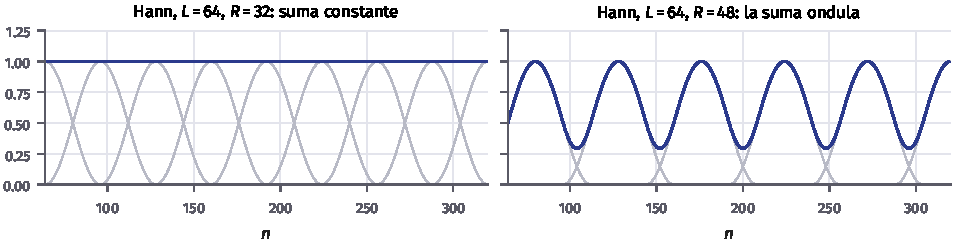
\includegraphics[width=\linewidth]{cola}
      \nota{Hann periódica: $w[n]=\frac12-\frac12\cos\frac{2\pi n}{L}$, $0\le n<L$.}
    \end{column}
  \end{columns}
  \herramienta{T5-stft}
\end{frame}

% =====================================================================
\section{Aplicaciones}

\begin{frame}{Ejemplo: marcación por tonos (DTMF)}
  \begin{columns}[c]
    \begin{column}{0.32\textwidth}
      \footnotesize
      \begin{itemize}
        \item Cada tecla suma un tono de fila (697, 770, 852, 941\,Hz) y uno de columna (1209, 1336, 1477\,Hz).
        \item El espectrograma muestra en qué instante se pulsa cada tecla y cuál es.
        \item $L=256$ a 8\,kHz son 32\,ms: basta para separar 697 y 770\,Hz ($2f_s/L=62{,}5$\,Hz) y es más corto que un tono.
      \end{itemize}
    \end{column}
    \begin{column}{0.66\textwidth}
      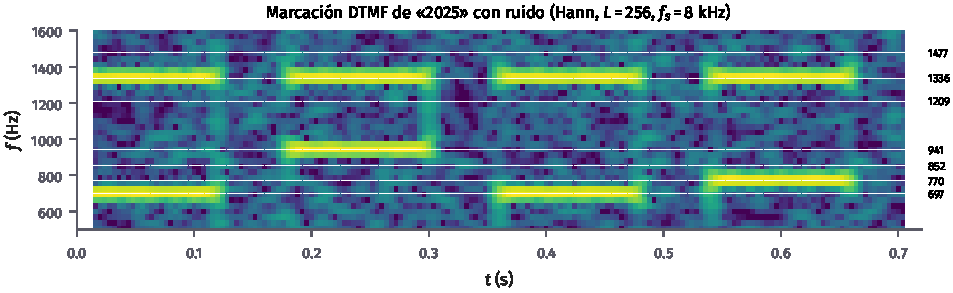
\includegraphics[width=\linewidth]{dtmf_espectrograma}
    \end{column}
  \end{columns}
  \herramienta{T5-dtmf}
\end{frame}

\begin{frame}{En código: reconocer una tecla}
  \codigo[basicstyle=\ttfamily\fontsize{6.3}{7.1}\selectfont]{dtmf}
  \nota{En la práctica se usa el algoritmo de Goertzel, que calcula solo las 7 frecuencias que interesan.}
\end{frame}

\begin{frame}{Otras aplicaciones}
  \begin{itemize}
    \item \alert{Voz}: los formantes y el tono se ven en el espectrograma; los reconocedores de voz parten de una STFT (coeficientes cepstrales en escala mel).
    \item \alert{Música}: identificar notas e instrumentos; \emph{vocoder} de fase para cambiar el tempo sin cambiar el tono.
    \item \alert{Vibraciones}: el arranque de un motor es un chirp; un rodamiento dañado produce armónicos que aparecen con el tiempo.
    \item \alert{Radar y sonar}: el desplazamiento Doppler a lo largo del tiempo.
    \item \alert{Reducción de ruido}: se atenúan los puntos del espectrograma donde domina el ruido y se resintetiza con solapamiento y suma.
  \end{itemize}
\end{frame}

% =====================================================================
\section*{Resumen}
\begin{frame}{Conceptos importantes}
  \begin{columns}[T]
    \begin{column}{0.5\textwidth}
      \begin{itemize}
        \item La DFT de toda la señal no dice cuándo aparece cada frecuencia.
        \item STFT: DFT de tramos enventanados; función de tiempo y frecuencia.
        \item Espectrograma: $\abs{X[m,k]}^2$ en dB sobre el plano tiempo-frecuencia.
      \end{itemize}
    \end{column}
    \begin{column}{0.5\textwidth}
      \begin{itemize}
        \item Parámetros: $L$, ventana, salto $R$, $N$. $M=\lfloor(N_x-L)/R\rfloor+1$ tramos.
        \item Compromiso: $\Delta t=L/f_s$, $\Delta f\sim f_s/L$.
        \item COLA: las ventanas desplazadas suman una constante; permite resintetizar.
      \end{itemize}
    \end{column}
  \end{columns}
  \bigskip
  \gris{Apuntes del Tema 5, sección 1 · Hoja de ejercicios, ejercicios 1–5.}
\end{frame}

\end{document}
